\documentclass[a4paper,12pt]{article}

\usepackage{a4wide}
\usepackage{amsmath}
\usepackage{amssymb}
\usepackage{amsthm}
\usepackage[czech]{babel}
\usepackage{bookmark}
\usepackage{enumerate}
\usepackage[T1]{fontenc}
\usepackage{forest}
\usepackage{hyperref}
\usepackage[utf8]{inputenc}
\usepackage{lmodern}
\usepackage{multicol}
\usepackage{tikz}

\theoremstyle{definition}
    \newtheorem{problem}{Příklad}

% \theoremstyle{remark}
%     \newtheorem*{steps}{Postup řešení}

\theoremstyle{plain}
    \newtheorem*{solution}{Řešení}
    

\DeclareRobustCommand\proves{\mathrel{|}\joinrel\mkern-.5mu\mathrel{-}}
\DeclareMathOperator{\Conseq}{Csq}
\DeclareMathOperator{\M}{M}

% hide solutions
\newif\ifhidesolutions
    \hidesolutionstrue
    % \hidesolutionsfalse

\ifhidesolutions
    \usepackage{environ}
    \NewEnviron{hide}{}
    \let\solution\hide
    \let\endsolution\endhide
\fi









\begin{document}

\section*{NAIL062 V\&P Logika: 5. cvičení}
% po 4. přednášce


\textbf{Témata:} 
Algoritmus DPLL. Kódování problémů do SAT. Tablo metoda ve výrokové logice. 


\medskip\begin{problem}
    Pomocí algoritmu DPLL rozhodněte, zda je následující CNF formule splnitelná.
    \begin{enumerate}
        \item $$ (\neg p_1 \wedge \neg p_2)\land( \neg p_1 \wedge p_2)\land( p_1 \wedge \neg p_2)\land( p_2 \wedge \neg p_3)\land( p_1 \wedge p_3)$$
        \item \begin{align*}
            &(\neg p_1 \wedge p_3 \wedge p_4)\vee( \neg p_2 \wedge p_6 \wedge p_4)\vee( \neg p_2 \wedge \neg p_6 \wedge \neg p_3)\vee(
                \neg p_4 \wedge \neg p_2)\vee \\ & ( p_2 \wedge \neg p_3 \wedge \neg p_1)\vee ( p_2 \wedge p_6 \wedge p_3)\vee
                ( p_2 \wedge \neg p_6 \wedge \neg p_4)\vee
                ( p_1 \wedge p_5)\vee \\ & ( p_1 \wedge p_6)\vee(
                \neg p_6 \wedge p_3 \wedge \neg p_5)\vee( p_1 \wedge \neg p_3 \wedge \neg p_5)    
        \end{align*}
    \end{enumerate}
\end{problem}


% \medskip\begin{problem}
%     Lze šachovnici $4\times 4$ bez dvou protilehlých rohů perfektně pokrýt kostkami domina? Zakódujte tento problém do SAT. Zobecněte na všechna sudá~$n$.
%     \end{problem}
        
        
    \medskip\begin{problem}
        Lze obarvit čísla od 1 do $n$ dvěma barvami tak, že neexistuje monochromatické řešení rovnice
        $a+b=c$ pro žádná $1\leq a<b<c\leq n$? Sestrojte výrokovou formuli $\varphi_n$ v CNF která je splnitelná, právě když to lze. Zkuste nejprve $n=8$.
        
        Zkuste si doma: Napište skript generující $\varphi_n$ v DIMACS CNF formátu. Použijte SAT solver k nalezení nejmenšího $n$ pro které takové obarvení neexistuje (tj. každé 2-obarvení obsahuje monochromatickou trojici $a<b<c$ takovou, že $a+b=c$).
    \end{problem}
    
        
    \medskip\begin{problem}
        Zakódujte problém setřídění trojice celých čísel do SAT.
    \end{problem}
        
            
    \medskip\begin{problem}
    Věta o čtyřech barvách říká, že následující mapy lze obarvit 4 barvami tak, že žádné dva sousedící regiony nemají stejnou barvu. Najděte takové obarvení pomocí SAT solveru.
    \begin{multicols}{2}
    \begin{enumerate}
        \item Mapa krajů Česka  
        
        \vfill 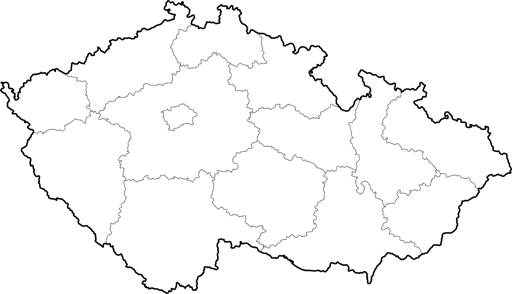
\includegraphics[width=0.5\textwidth]{files/map-coloring-czechia.png} \vfill
        
        \item Těžší instance  
        
        \vfill 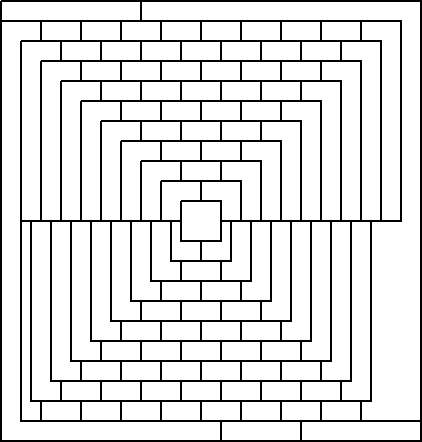
\includegraphics[width=0.33\textwidth]{files/map-coloring-hard.png} \vfill
    \end{enumerate}
    \end{multicols}
    \end{problem}
    
    
\newpage   


\medskip\begin{problem}
    Pomocí tablo metody dokažte následující výroky:
    \begin{enumerate}
    \item $(p\to (q \to q))$
    \item $p \leftrightarrow \neg \neg  p$
    \item $\neg (p \vee q) \leftrightarrow (\neg p \wedge \neg q)$
    \item $(p \to q) \leftrightarrow (\neg q \to \neg p)$    
    \end{enumerate}
\end{problem} 
   

\medskip\begin{problem}
    Pomocí tablo metody dokažte nebo najděte protipříklad ve formě \emph{kanonického} modelu pro bezespornou větev.
    \begin{enumerate}
    \item $\{ \neg q,\ p \vee q\} \models p$
    \item $\{ q \to p,\ r \to q,\ (r \to p) \to s\} \models s$
    \item $\{ p \to r,\ p \vee q,\ \neg s \to \neg q\} \models r \to s$
    \end{enumerate}
\end{problem}
  

\medskip\begin{problem}
    Pomocí tablo metody určete všechny modely následujících teorií:
    \begin{enumerate}
    \item $\{(\neg p \vee q) \to (\neg q \wedge r)\}$
    \item $\{\neg q \to (\neg p \vee q),\ \neg p \to q,\ r \to q\}$
    \item $\{ q \to p,\ r \to q,\ (r \to p) \to s\}$
    \end{enumerate}
\end{problem}


\end{document}